\documentclass{chi-ext}

\copyrightinfo{
  Copyright is held by the author/owner(s).\\
  \emph{CHI'12}, May 5--10, 2012, Austin, Texas, USA.\\
  ACM 978-1-4503-1016-1/12/05.\\
}

\title{SkruiFab: A Sketch-based tool for making precise drawings for
  laser cutters}

\numberofauthors{2}
% Notice how author names are alternately typesetted to appear ordered
% in 2-column format; i.e., the first 4 autors on the first column and
% the other 4 auhors on the second column.  Actually, it's up to you
% to strictly adhere to this author notation.
\author{
  \alignauthor{
  	\textbf{First Author}\\
  	\affaddr{AuthorCo, Inc.}\\
  	\affaddr{Authortown, PA 54321 USA}\\
  	\email{author1@anotherco.com}
  }\alignauthor{
  	\textbf{Second Author}\\
  	\affaddr{AuthorCo, Inc.}\\
  	\affaddr{123 Author Ave.}\\
  	\email{author2@anotherco.com}
  }
}

\teaser{
  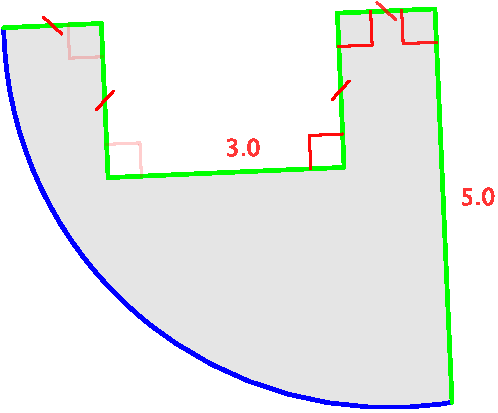
\includegraphics[width=0.8\columnwidth]{img/skruifab-sample-screen.pdf}
  \caption{SkruiFab enables users to quickly create precise vector
    drawings like this using sketch-based interaction.}
  \label{fig:sample}
}

% Paper metadata (use plain text, for PDF inclusion and later
% re-using, if desired)
\def\plaintitle{Metadata Title Here} 

\def\plainauthor{Gabe Johnson}

\def\plainkeywords{comma, separated, keywords, here}

\def\plaingeneralterms{General, Terms, Here}

\hypersetup{
  % Your metadata go here
  pdftitle={\plaintitle},
  pdfauthor={\plainauthor},  
  pdfkeywords={\plainkeywords},
  pdfsubject={\plaingeneralterms},
  % Quick access to color overriding:
  citecolor=black,
  linkcolor=blue,
  menucolor=black,
  urlcolor=blue,
}

\usepackage{graphicx}   % for EPS use the graphics package instead
\usepackage{balance}    % useful for balancing the last columns
\usepackage{bibspacing} % save vertical space in references

% ----------------------------------------------------------------------

\begin{document}

\maketitle

\begin{abstract}
SkruiFab is a modeling tool that enables non-experts to design items
for fabrication with laser cutters. Users provide rough, freehand
input that is recognized to iteratively edit a structured vector
drawing. 
\end{abstract}

\keywords{\plainkeywords}
% Get CHI keywords and put them here.
\category{H.5.m}{Information interfaces and presentation (e.g.,
  HCI)}{Miscellaneous}.


% ======================================================================
\section{Introduction}
% ======================================================================

Rapid fabrication machines such as laser cutters and 3D printers allow
people to make things that would otherwise be too difficult or time
consuming to build. Such machines are becoming more common as their
quality improves and their cost declines. The availability of these
machines is closely associated with an increasingly popular culture of
making. Unfortunately, users often have difficulty using the design
software associated with this activity.

Today's design/build process typically begins with sketching on paper,
followed by a session with a computer tool. Eventually, the rapid
fabrication machinery is set to work. 

In recent years, computational support for sketching has focused
mostly on the early phases of design. This is for good reason: paper
and pencil sketching remain central to design practice despite the
ubiquity of powerful computer-based design tools. Ideas that begin as
rough sketches may eventually be made with rapid fabrication machines.


\begin{figure}
\hspace*{-0.4\columnwidth}% displace figure
\parbox{1.4\columnwidth}{
  \centering
  \includegraphics[width=1.4\columnwidth]{sample.jpg}
  \caption{Insert a caption below each figure. Images can "float" around body text, like this example.}
  \label{fig:sample}
}
\end{figure}

% =============================================================================
\section{A section...}
% =============================================================================
More text goes here. More text goes here. More text goes here. More
text goes here. More text goes here. More text goes here. More text
goes here. More text goes here. More text goes here. More text goes
here. More text goes here. More text goes here. More text goes
here. More text goes here. More text goes here. More text goes
here. More text goes here. More text goes here. More text goes
here. More text goes here. More text goes here. More text goes
here. More text goes here. More text goes here. More text goes
here. More text goes here. More text goes here. More text goes
here. More text goes here. More text goes here. More text goes
here. More text goes here.

More text goes here. More text goes here. More text goes here. More
text goes here. More text goes here. More text goes here. More text
goes here. More text goes here. More text goes here. More text goes
here. More text goes here. More text goes here. More text goes
here. More text goes here. More text goes here.

\subsection{A subsection here...}
% -----------------------------------------------------------------------------
Subsection text here. Subsection text here. Subsection text
here. Subsection text here. Subsection text here. Subsection text
here. Subsection text here. Subsection text here. Subsection text
here. Subsection text here. Subsection text here. Subsection text
here. Subsection text here. Subsection text here. Subsection text
here. Subsection text here. Subsection text here. Subsection text
here. Subsection text here. Subsection text here. Subsection text
here. Subsection text here. Subsection text here.

% =============================================================================
\section{A section...}
% =============================================================================
More text goes here. More text goes here. More text goes here. More
text goes here. More text goes here. More text goes here. More text
goes here. More text goes here. More text goes here. More text goes
here. More text goes here. More text goes here. More text goes
here. More text goes here. More text goes here. More text goes
here. More text goes here. More text goes here. More text goes
here. More text goes here. More text goes here. More text goes
here. More text goes here. More text goes here. More text goes
here. More text goes here. More text goes here. More text goes
here. More text goes here. More text goes here. More text goes
here. More text goes here.

More text goes here. More text goes here. More text goes here. More
text goes here. More text goes here. More text goes here. More text
goes here. More text goes here. More text goes here. More text goes
here. More text goes here. More text goes here. More text goes
here. More text goes here. More text goes here.

\subsection{A subsection here...}
% -----------------------------------------------------------------------------
Subsection text here. Subsection text here. Subsection text
here. Subsection text here. Subsection text here. Subsection text
here. Subsection text here. Subsection text here. Subsection text
here. Subsection text here. Subsection text here. Subsection text
here. Subsection text here. Subsection text here. Subsection text
here. Subsection text here. Subsection text here. Subsection text
here. Subsection text here. Subsection text here. Subsection text
here. Subsection text here. Subsection text here.

% =============================================================================
\section{A section...}
% =============================================================================
More text goes here. More text goes here. More text goes here. More
text goes here. More text goes here. More text goes here. More text
goes here. More text goes here. More text goes here. More text goes
here. More text goes here. More text goes here. More text goes
here. More text goes here. More text goes here. More text goes
here. More text goes here. More text goes here. More text goes
here. More text goes here. More text goes here. More text goes
here. More text goes here. More text goes here. More text goes
here. More text goes here. More text goes here. More text goes
here. More text goes here. More text goes here. More text goes
here. More text goes here.

More text goes here. More text goes here. More text goes here. More
text goes here. More text goes here. More text goes here. More text
goes here. More text goes here. More text goes here. More text goes
here. More text goes here. More text goes here. More text goes
here. More text goes here. More text goes here.

\subsection{A subsection here...}
% -----------------------------------------------------------------------------
Subsection text here. Subsection text here. Subsection text
here. Subsection text here. Subsection text here. Subsection text
here. Subsection text here. Subsection text here. Subsection text
here. Subsection text here. Subsection text here. Subsection text
here. Subsection text here. Subsection text here. Subsection text
here. Subsection text here. Subsection text here. Subsection text
here. Subsection text here. Subsection text here. Subsection text
here. Subsection text here. Subsection text here.

% =============================================================================
\section{Image section}
% =============================================================================

There are images here. There are images here. There are images
here. There are images here. There are images here. There are images
here. There are images here. There are images here. There are images
here. There are images here. There are images here. There are images
here. There are images here. There are images here.

\begin{figure}
%\hspace*{-0.5\textwidth}% displace figure
\parbox{\textwidth}{
  \begin{center}
  \frame{\includegraphics[width=\textwidth]{sample.jpg}}
  \caption{A big figure. You may want to place some marginal notes in this page, as shown above. Notice also that this image resolution is quite low, as it is just an example of formatting.}
  \label{fig:bigsample}
  \end{center}  
}
\end{figure}

\balance
\bibliographystyle{acm-sigchi}
\bibliography{sample}

\end{document}
